\chapter{Administrátorské rozhraní}
\label{4-praxe}

\begin{figure}[H] \centering
    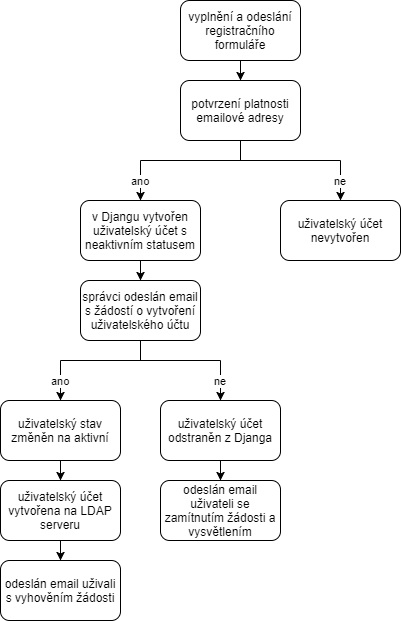
\includegraphics[width=250pt]{./pictures/my_console_final_version_cz.png}
    \caption[Vytváření uživatele - finální stav]{Vytváření uživatele - finální stav (zdroj:
	\href{}{Tereza Kulovaná})}
    \label{fig:admin-final}
  \end{figure}

\begin{figure}[H] \centering
    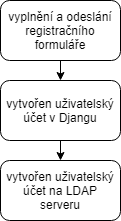
\includegraphics[width=70pt]{./pictures/my_console_current_version_cz.png}
    \caption[Vytváření uživatele - současný stav]{Vytváření uživatele - současný stav (zdroj:
	\href{}{Tereza Kulovaná})}
    \label{fig:admin-current}
  \end{figure}

\section{Současná správa uživatelských účtů}
\label{cmd-line}
% https://github.com/gislab-npo/gislab/tree/314fe436e1b65783d65e61000ca6d3f8ba873b2f/system/admin

Aktuálně probíhá správa uživatelských účtů spouštěním shellových skriptů. Všechny příkazy je nutné spouštět pod právem \textit{sudo}. Některé z nich umožňují použití parametrů, pro část jsou dokonce povinné.

Seznam názvů dostupných skriptů pro GIS.lab administraci vrací příkaz \texttt{gislab-help}. Každý jednotlivý příkaz z tohoto soupisu pak lze spustit s příznakem \texttt{-h}, který zobrazí podrobnější nápovědu. Uživatel se dozví, co skript vykoná a za jakých podmínek, jakým způsobem příkaz zapsat do konzole a získá přehled parametrů, které může či musí použít.

Níže jsou popsány skripty pro vytváření uživatelů a skupin, jejich mazání a pro výpis existujících entit, protože souvisí s funkčností, kterou nabízí nové webové rozhraní. Vedle toho existují i další, např. pro zálohování dat nebo upgrade GIS.lab systému.

%TK: tady u těch popisů nevím, jestli dávat někam přesnou podobu příkazu (gislab-adduser [OPTIONS] username)
%přímo jako nadpis (\subsubsection{gislab-adduser...}) nebo někam pod něj? nebo to nepsat vůbec?
%nebo mít u každého konkrétní příkaz: $ sudo gislab-adduser -g User -l GIS.lab -m lab1@gis.lab -p lab lab1 ??

\subsubsection{gislab-adduser}
\begin{itemize}
\item [-g] křestní jméno (povinné)
\item [-l] příjmení (povinné)
\item [-m] email (povinné)
\item [-d] popis (nepovinné)
\item [-p] heslo (nepovinné)
\item [-s] přidat uživateli status administrátora (nepovinné)
\item [-a] přidat uživatele do vybraných skupin (nepovinné)
\end{itemize}
Tento příkaz má několik příznaků, z nichž část je povinná, část nepovinná. Parametr \texttt{-p} musí být použit jako poslední, těsně před názvem uživatele (username), může však být aplikován v různých obměnách. První variantou je \texttt{-p PASSWORD}, která nastaví heslo na hodnotu PASSWORD. Pokud je použit parametr bez argumentu (\texttt{-p}), uživatel je následně dotázán na heslo. V třetím případě je parametr z příkazu kompletně vynechán a heslo je automaticky vygenerováno. Tedy i přestože parametr patří mezi nepovinné, heslo je vždy po doběhnutí skriptu vytvořeno.

Uživatele lze přidat do více skupin zároveň použitím parametru \texttt{-a} a seznamu skupin oddělených od sebe čárkami. Pokud je k účtu přiřazen status administrátora (superuser), tak takový uživatel může na klientských počítačích spouštět operace pod právem \textit{sudo}.

\subsubsection{gislab-moduser}
\begin{itemize}
\item [-a] přidat uživatele do vybrané skupiny
\item [-A] odebrat uživatele z vybrané skupiny
\item [-s] přidat uživateli status administrátora
\item [-S] odebrat uživateli status administrátora
\item [-m] změnit email
\item [-p] změnit heslo
\item [-d] změnit popis
\end{itemize}
Upraví jeden či více atributů. Pokud nebyly předtím definovány, tak je vytvoří. Stejně jako při vytváření uživatelského účtu je možné přidávat a odebírat členství ve skupinách hromadně, jsou-li v seznamu a oddělené čárkami. V případě, že je parametr \texttt{-p} uveden bez argumentu, je heslo vygenerováno automaticky.

\subsubsection{gislab-deluser}
\begin{itemize}
\item [-b] zazálohovat uživatelská data (nepovinné)
\item [-f] vynutit proběhnutí tohoto příkazu (nepovinné)
\end{itemize}
Smaže uživatelský účet včetně příslušnosti ke skupinám. Pokud je příkaz spuštěn s parametrem \texttt{-f}, proběhne vše okamžitě, v opačném případě musí uživatel ještě jednou potvrdit, že si skutečně přeje účet odstranit.

\subsubsection{gislab-addgroup}
\begin{itemize}
\item [-d] popis (nepovinné)
\end{itemize}
Vytvoří skupinu.

\subsubsection{gislab-delgroup}
\begin{itemize}
\item [-f] vynutit proběhnutí tohoto příkazu
\end{itemize}
Smaže skupinu, pokud je prázdná. Existují-li uživatelé, kteří patří do mazané skupiny, vypíše se chybová hláška a skupina zůstane v systému. Nejdříve je potřeba skupinu vyčistit přes \texttt{gislab-moduser} a pak příkaz zopakovat.

Obdobně jako při mazání uživatelského účtu je možné vynutit proběhnutí příkazu bez dalších dotazů. Pokud však zůstali nějací uživatelé ve skupině, je vrácena stejná chyba, která byla popsána výše.

\subsubsection{gislab-listusers}
\begin{itemize}
\item [-g] vypsat pouze uživatele zvolené skupiny
\end{itemize}
Bez příznaku vypíše seznam všech uživatelů. U každého uživatele jsou uvedeny všechny jeho atributy. S příznakem \texttt{-g nazev\_skupiny} vypíše list uživatelů příslušících této skupině, včetně jejich atributů. Heslo je zobrazeno v šifrované podobě. 

\subsubsection{gislab-listgroups}
Kromě nápovědy nemá žádné parametry. Vypíše seznam všech skupin a jejich atributů, včetně identifikátorů \textit{uid} uživatelů, kteří do dané skupiny patří. 

Jak \texttt{gislab-listusers}, tak \texttt{gislab-listgroups} vracejí při větším množství záznamů velmi dlouhý seznam, který vypisují do konzole. Zobrazit jen požadovanou část informací umožňuje program grep.

\texttt{\$ sudo gislab-listusers | grep uid:}

\texttt{uid: uid=user01}

\texttt{uid: uid=user02}

%TK: u listusers a listgroups by možná pro lepší orientaci pomohlo přidat obrázky nebo textový výpis, jak vlastně vypadají výsledky, které vrací:
%dn: uid=gislab,ou=People,dc=gis,dc=lab                                                                                  objectClass: inetOrgPerson                                                                                              objectClass: posixAccount                                                                                               objectClass: shadowAccount                                                                                              uid: gislab                                                                                                             uidNumber: 3000                                                                                                         gidNumber: 3001                                                                                                         homeDirectory: /mnt/home/gislab                                                                                         loginShell: /bin/bash                                                                                                   cn: Administrator GIS.lab (gislab_vagrant_bionic)                                                                       sn: GIS.lab (gislab_vagrant_bionic)                                                                                     givenName: Administrator                                                                                                mail: gislab@gis.lab                                                                                                    userPassword:: e1NTSEF9Y0JBWUdMcVgxNTdweVJreXdxZzJRaUlpTE9CaHNaSTU=                                                     description: fjdsklfjdsl 

\section{Webové administrátorské rozhraní}
spíš z technického hlediska a implementace
(z uživatelského pak jako příloha)

Pro vývoj webové administrátorské konzole byl využit odlehčený webový server Djanga (vývojový server).

\subsection{Struktura projektu}
%popsat strukturu celé aplikace, jednotlivé soubory a třídy
Adresářová struktura projektu:
% tomuhle budu chtít dát hezčí design
% např. forest: https://tex.stackexchange.com/questions/5073/making-a-simple-directory-tree
% https://tex.stackexchange.com/questions/328886/making-a-directory-tree-of-folders-and-files/328890
\dirtree{%
.1 web\_admin\_console.			
	.2 project.
		.3 \_\_init\_\_.py.
		.3 ldap\_auth.py.
		.3 settings.py.
		.3 settings\_custom.py.
		.3 urls.py.
		.3 wsgi.py.
    .2 static.
    	.3 styles.css.
	.2 templates.
		.3 registration.
			.4 login.html.
		.3 base.html.
		.3 home.html.
		.3 password\_change.html.
		.3 signup.html.
		.3 user\_change.html.
	.2 users.
		.3 templatetags.
			.4 \_\_init\_\_.py.
			.4 auth\_extras.py.
		.3 \_\_init\_\_.py.
		.3 admin.py.
		.3 apps.py.
		.3 forms.py.
		.3 ldap\_sync.py.
		.3 models.py.
		.3 tests.py.
		.3 urls.py.
		.3 views.py.
	.2 db.sqlite3.
	.2 manage.py.
    }
% popsat jen ty nejdůležitější soubory


\subsubsection{project}

\subsubsection{templates, templatetags, static}
Složka \textit{templates} obsahuje šablony (templates), psané v jazyce \zk{HTML}, které umožňují vypisovat vybraná data z modelů do prohlížeče. Cesta k adresáři musí být registrována v souboru \textit{settings.py} v proměnné \texttt{DIRS} u položky \texttt{TEMPLATES}.

Pro přístup k proměnným a některým funkcím Pythonu slouží složené závorky. V případě proměnných se jedná o závorky dvojité: \texttt{\{\{ variable \}\}}. 

%popis sablon
Django funguje na principu dědičnosti. Bázovou šablonou je \textit{base.html}. Vložením textu \texttt{\{\% extends "base.html" \%\}} na začátek jiné šablony, např. \textit{child.html}, je nejdříve načtena šablona \textit{base.html}, definující základní bloky, a až následně je k nim přidán obsah \textit{child.html}. Tímto způsobem jsou omezeny duplicity v jednotlivých šablonách.

U tohoto projektu jsou například v bázové šabloně definovány navigační prvky společné pro níže uvedené šablony, které z ní všechny dědí. Na každé stránce se v horní části zobrazuje logo GIS.labu, které po kliknutí přesměruje uživatele na hlavní stránku \textit{home.html}. V případě přihlášeného uživatele se navíc zobrazuje tlačítko pro odhlášení.

\textit{signup.html} obsahuje jednoduchý interaktivní formulář s informacemi, která pole jsou povinná pro platné vyplnění a jaké podmínky musí splňovat. V situaci, kdy je registrace provedena správně, je uživatel přesměrován na přihlašovací stránku, v opačném případě je zobrazena chybová hláška a potřebná data je nutné opravit, resp. doplnit.

Template \textit{login.html} sestává z jednoduchého formuláře pro vyplnění uživatelského jména a hesla. Při neúspěšném pokusu je vypsána chyba, po zdárném vyplnění je uživatel přesměrován na domovskou stránku \textit{home.html}.

První šablona, s níž se uživatel při zobrazení hlavní stránky setká, je \textit{home.html}. Ta ukazuje rozdílné výsledky nepřihlášenému uživateli a přihlášenému. V prvním případě je dostupný rozcestník, který jej navede na stránky přihlášení či k registraci. V druhém případě, tedy pokud je již přihlášen, se zobrazí jeho osobní informace a aktivní role. Přímo zde nemůže nic upravovat, ale pomocí tlačítka \texttt{Edit} je přesměrován na stránku s úpravou osobních údajů.

Šablona \textit{user\_change.html} obsahuje formulář pro editaci osobních údajů, který umožňuje upravit jeden či více záznamů naráz. Heslo se zde nezobrazuje, ale přes odkaz lze pokračovat na stránku \textit{password\_change.html}, kde je možné provést jeho změnu.

%static
Složka \textit{static} umístěná v hlavním adresáři projektu obsahuje soubor \textit{styles.css}, jenž popisuje způsob zobrazení elementů, které jsou součástí jednotlivých šablon uživatelské konzole. To je umožněno načtením tohoto souboru pomocí \texttt{\{\% load static \%\}} do bázové šablony. K vytvoření designu byly použity kaskádové styly (\zk{CSS}).

%template tags
Django umožňuje vytvořit si vlastní filtry. Ty jsou specifikovány v souboru \textit{auth\_extras.py} uloženém v adresáři aplikace \textit{users/templatetags} a k šablonám jsou připojeny pomocí \texttt{\{\% load auth\_extras \%\}}. Filtru \texttt{foo} lze předat hodnotu proměnné \textit{var} a argument \textit{arg}. Poté, co je filtr zaregistrován jako \textit{django.template.Library.filter()} a definována žádaná funkce, je možné jej zavolat v šabloně příkazem:

\texttt{\{\{ var|foo:"arg" \}\}}

Pro potřeby zobrazení aktivních rolí uživatele v šabloně \textit{home.html} byly vytvořeny dva filtry. První zjišťuje všechny existující role v databázi Djanga a na něj navazuje druhý, který určuje, zda je uživatel jejich členem. Výsledky jsou pak zobrazeny v \zk{GUI}.

\subsubsection{users}

\subsubsection{db.sqlite3}
% https://www.tablesgenerator.com/latex_tables

Pro vývoj byla využita implicitní databáze Djanga SQLite. 
Z hlediska uživatelů a rolí jsou důležité především tři tabulky \textit{auth\_group}, \textit{users\_customuser} a \textit{users\_customuser\_groups}. 

Tabulka \textit{auth\_group} obsahuje pouze názvy existujících rolí.

\begin{table}[H]
\centering
\begin{tabular}{@{}|c|c|c|@{}}
\toprule
\multicolumn{3}{|c|}{auth\_group} \\ \midrule
name & id & name \\ \midrule
type & integer & varchar(80) \\ \bottomrule
\end{tabular}
\caption{Atributy tabulky auth\_group}
\label{tab:auth-group}
\end{table}

Tabulka \textit{users\_customuser} sestává z osobních údajů uživatelů včetně zašifrovaného hesla, data vytvoření, posledního přihlášení a interních statusů Djanga. 

\begin{table}[H]
\centering
\resizebox{\textwidth}{!}{%
\begin{tabular}{@{}|c|c|c|c|c|c|c|@{}}
\toprule
\multicolumn{7}{|c|}{users\_customuser} \\ \midrule
name & id & password & last\_login & is\_superuser & username & first\_name \\ \midrule
type & integer & varchar(128) & datetime & bool & varchar(150) & varchar(30) \\ \bottomrule
\end{tabular}%
}
\caption{Atributy tabulky users\_customuser 1/2}
\label{tab:users-customuser-1}
\end{table}

\begin{table}[H]
\centering
\resizebox{\textwidth}{!}{%
\begin{tabular}{@{}|c|c|c|c|c|c|c|@{}}
\toprule
\multicolumn{7}{|c|}{users\_customuser} \\ \midrule
name & last\_name & email & is\_staff & is\_active & date\_joined & description \\ \midrule
type & varchar(150) & varchar(254) & bool & bool & datetime & text \\ \bottomrule
\end{tabular}%
}
\caption{Atributy tabulky users\_customuser 2/2}
\label{tab:users-customuser-2}
\end{table}

Tabulka \textit{users\_customuser\_groups} propojuje obě výše zmíněné tabulky, tj. příslušnost uživatelů k jednotlivým skupinám.

\begin{table}[H]
\centering
\begin{tabular}{@{}|c|c|c|c|@{}}
\toprule
\multicolumn{4}{|c|}{users\_customuser\_groups} \\ \midrule
name & id & customuser\_id & group\_id \\ \midrule
type & integer & integer & integer \\ \bottomrule
\end{tabular}
\caption{Hlavička tabulky users\_customuser\_groups}
\label{tab:users-customuser-groups}
\end{table}

\subsection{problémy při zpracování}

\subsection{co přibude do budoucna}
\label{python-knihovna}


